\externaldocument{proj_paper}
\section{Methodology}
Our method for checking what operating system a host is using involved an analysis of packets. By analyzing the first packet of a TCP session, we can make a good guess of the operating system based on a few traits in the packet header.

\subsection{Packet Analysis}
Explain how packets have a specific structure based on the protocol.

\subsubsection{Window Size}
What is Window Size? Where is it stored in the packet? How did we use it to our advantage?

''The TCP receive window size is the amount of receive data (in bytes) that can be buffered at one time on a connection. The sending host can send only that amount of data before waiting for acknowledgments for data sent and window updates from the receiving host. Windows 2000 TCP/IP is designed to tune itself in most environments, and uses larger default window sizes than earlier versions.''~\cite{Microsoft1}

\subsubsection{Time to Live}
What is TTL? Where is it stored in the packet? How did we use it to our advantage?

''Time-to-live (TTL) is a value in an Internet Protocol (IP) packet that tells a network router whether or not the packet has been in the network too long and should be discarded.'' ~\cite{Rouse07}

\begin{figure}[p]
	\center{\fbox{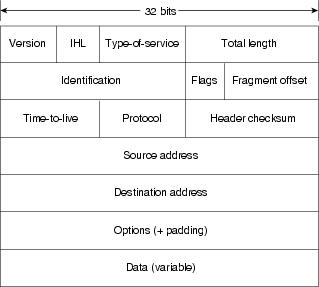
\includegraphics[width=.5\textwidth]
	{images/tcpdiagram.jpg}}}
	\caption{\label{fig:tcpDiagram} IP Packet Format~\cite{Cisco1}}
\end{figure}

\subsection{Implementation}
Talk about scapy~\cite{Scapy} and python~\cite{Python} here.
Go through code.

\begin{figure}[p]
	\center{\fbox{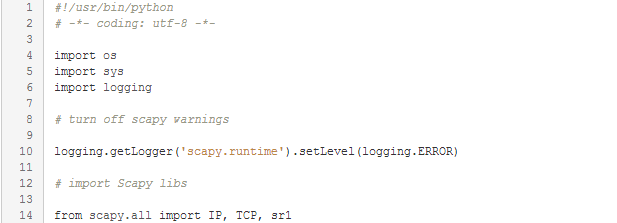
\includegraphics[width=\textwidth]
	{images/code1.png}}}
	\caption{\label{fig:setupCode} Setup Code}
\end{figure}

\begin{figure}[p]
	\center{\fbox{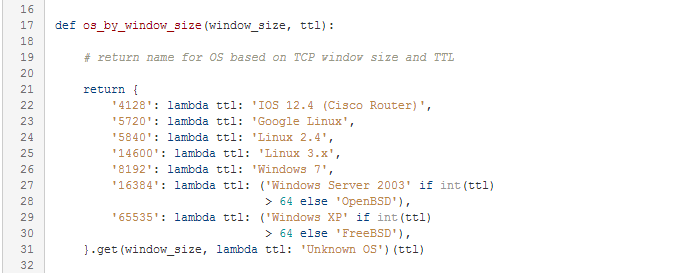
\includegraphics[width=\textwidth]
	{images/code2.png}}}
	\caption{\label{fig:osFunction} OS Identifier Function}
\end{figure}

\begin{figure}[p]
	\center{\fbox{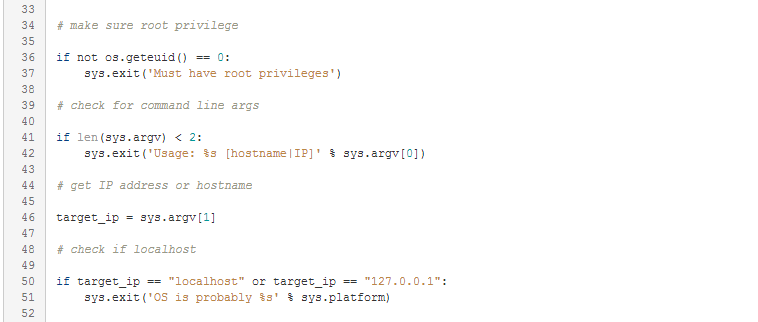
\includegraphics[width=\textwidth]
	{images/code3.png}}}
	\caption{\label{fig:prepare} Input and System Checks}
\end{figure}

\begin{figure}[p]
	\center{\fbox{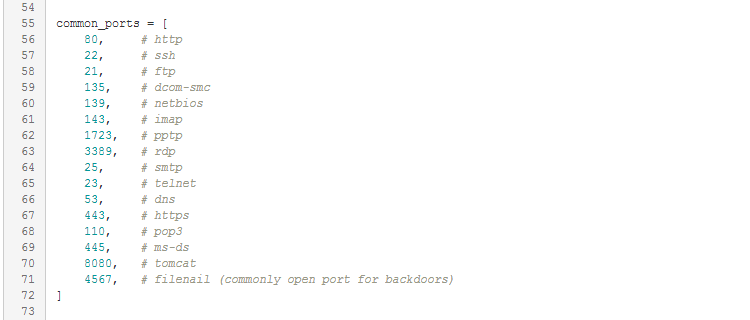
\includegraphics[width=\textwidth]
	{images/code4.png}}}
	\caption{\label{fig:ports} Array of Ports}
\end{figure}

\begin{figure}[p]
	\center{\fbox{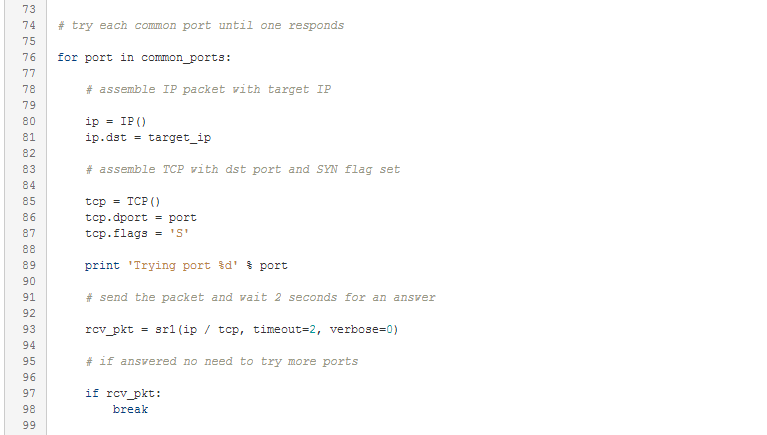
\includegraphics[width=\textwidth]
	{images/code5.png}}}
	\caption{\label{fig:loop} Packet Sending Loop}
\end{figure}

\begin{figure}[p]
	\center{\fbox{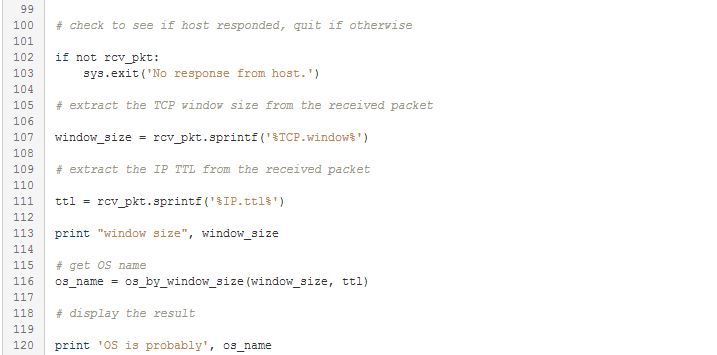
\includegraphics[width=\textwidth]
	{images/code6.png}}}
	\caption{\label{fig:results} Result Interpretation and Output}
\end{figure}

\subsection{Testing}
Figure~\ref{fig:testScript} shows the shell script we used to test the program.

\begin{figure}[h]
	\center{\fbox{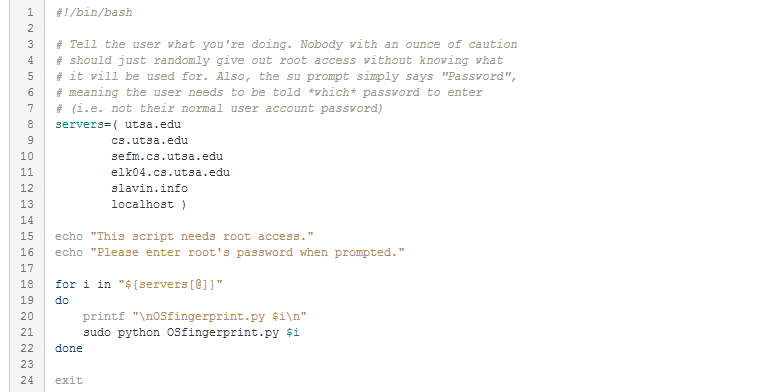
\includegraphics[width=\textwidth]
	{images/testCode.png}}}
	\caption{\label{fig:testScript} Testing Shell Script}
\end{figure}

\subsection{Results and Threats}
This might be better as a new section. Not sure if we'd have enough content for it, though.